\subsection{Упражнение 1}

Измените пример в chap10.ipynb и убедитесь, что дополнение нулями устраняет лишнюю ноту в начале фрагмента:

Устраним проблему с лишней нотой путем добавления нулей в конец сигнала.

\begin{lstlisting}[language=Python]
from thinkdsp import read_wave

response = read_wave('180960__kleeb__gunshot.wav')
start = 0.12
response = response.segment(start=start)
response.shift(-start)
response.normalize()
response.plot()
decorate(xlabel='Time (s)')
\end{lstlisting}
\begin{figure}[H]
	\begin{center}
		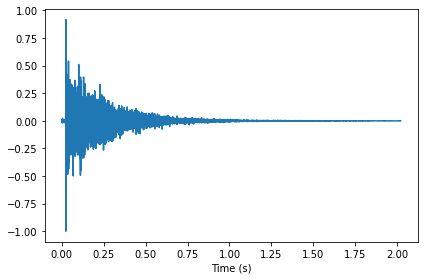
\includegraphics[scale=1]{fig/lab10/lab10_1.png}
		\caption{Сигнал}
	\end{center}
\end{figure}

\begin{lstlisting}[language=Python]
spec = response.make_spectrum()
spec.plot()
decorate(xlabel='Frequency (Hz)', ylabel='Amplitude')
\end{lstlisting}
\begin{figure}[H]
	\begin{center}
		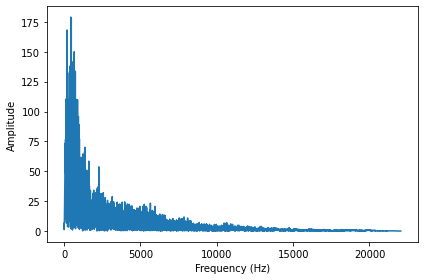
\includegraphics[scale=1]{fig/lab10/lab10_2.png}
		\caption{Спектр сигнала}
	\end{center}
\end{figure}

Теперь перейдём к самой записе:

\begin{lstlisting}[language=Python]
violin = read_wave('92002__jcveliz__violin-origional.wav')
start = 0.11
violin = violin.segment(start=start)
violin.shift(-start)
violin.truncate(len(response))
violin.normalize()
violin.plot()
decorate(xlabel='Time (s)')
\end{lstlisting}
\begin{figure}[H]
	\begin{center}
		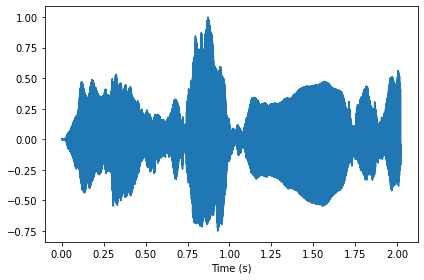
\includegraphics[scale=1]{fig/lab10/lab10_3.png}
		\caption{График сигнала}
	\end{center}
\end{figure}

\begin{lstlisting}[language=Python]
spec2 = violin.make_spectrum()
\end{lstlisting}

Теперь умножим ДПФ сигнала на передаточную функцию и преобразуем обратно в волну.

\begin{lstlisting}[language=Python]
wave = (spec * spec2).make_wave()
wave.normalize()
wave.plot()
\end{lstlisting}
\begin{figure}[H]
	\begin{center}
		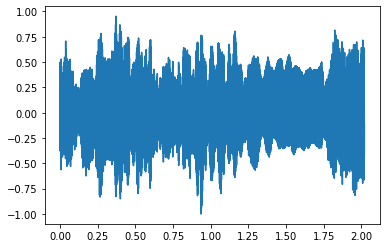
\includegraphics[scale=1]{fig/lab10/lab10_4.png}
		\caption{График получившегося сигнала}
	\end{center}
\end{figure}

Проблему удалось решить.

\subsection{Упражнение 2}

Необходимо смоделировать двумя способами звучание записи в том пространстве, где была измерена импульсная харпактеристика, как свёрткой самой записи с импульсной характеристикой, так и умножением ДПФ записи на вычисленный фильтр, соотвествующий импульсной характеристики. Характеристику возьмем из учебника.


\begin{lstlisting}[language=Python]
if not os.path.exists('stalbans_a_mono.wav'):
    !wget https://github.com/AllenDowney/ThinkDSP/raw/master/code/stalbans_a_mono.wav

response = read_wave('stalbans_a_mono.wav')

start = 0
duration = 5
response = response.segment(duration=duration)
response.shift(-start)
response.normalize()
response.plot()
decorate(xlabel='Time (s)')
decorate(xlabel='Time (s)')
\end{lstlisting}
\begin{figure}[H]
	\begin{center}
		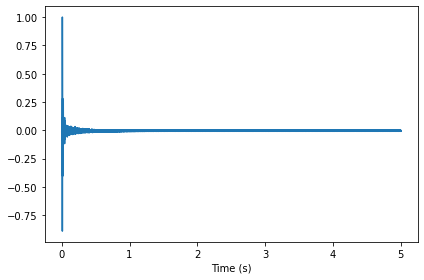
\includegraphics[scale=1]{fig/lab10/lab10_5.png}
		\caption{График загруженного сигнала}
	\end{center}
\end{figure}

ДПФ:

\begin{lstlisting}[language=Python]
transfer = response.make_spectrum()
transfer.plot()
\end{lstlisting}
\begin{figure}[H]
	\begin{center}
		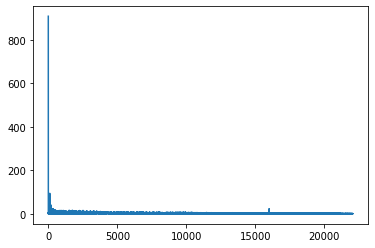
\includegraphics[scale=1]{fig/lab10/lab10_6.png}
		\caption{ДПФ импульсной характеристики}
	\end{center}
\end{figure}

Промоделируем запись в пространстве, будем также использовать звук из учебника - скрипку

\begin{lstlisting}[language=Python]
wave = read_wave('92002__jcveliz__violin-origional.wav')
start = 0.0
wave = wave.segment(start=start)
wave.shift(-start)
wave.truncate(len(response))
wave.normalize()
wave.plot()
\end{lstlisting}
\begin{figure}[H]
	\begin{center}
		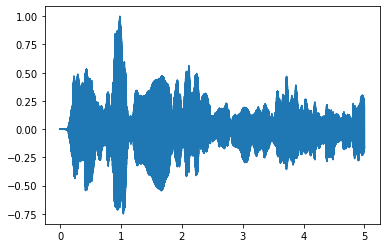
\includegraphics[scale=1]{fig/lab10/lab10_7.png}
		\caption{Сигнал звука скрипки}
	\end{center}
\end{figure}


\begin{lstlisting}[language=Python]
spectrum = wave.make_spectrum()
len(spectrum.hs), len(transfer.hs)
\end{lstlisting}
\begin{lstlisting}
(110251, 110251)
\end{lstlisting}

\begin{lstlisting}[language=Python]
spectrum.fs, transfer.fs
\end{lstlisting}
\begin{lstlisting}
(array([0.00000e+00, 2.00000e-01, 4.00000e-01, ..., 2.20496e+04,
        2.20498e+04, 2.20500e+04]),
 array([0.00000e+00, 2.00000e-01, 4.00000e-01, ..., 2.20496e+04,
        2.20498e+04, 2.20500e+04]))
\end{lstlisting}

Используем свертку.

\begin{lstlisting}[language=Python]
con = wave.convolve(response)
con.normalize()
con.make_audio()
\end{lstlisting}

Используем умножение:
\begin{lstlisting}[language=Python]
result = (spectrum * transfer).make_wave()
result.normalize()
result.plot()
\end{lstlisting}

\begin{figure}[H]
	\begin{center}
		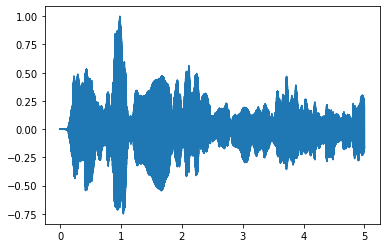
\includegraphics[scale=1]{fig/lab10/lab10_7.png}
		\caption{Полученный график}
	\end{center}
\end{figure}

\subsection{Вывод}

В данной работе мы рассмотрели основные позиции из теории сигналов и систем, например музыкальную акустику. При описании линейных стационарных систем используется теорема о свёртке.
